\documentclass[]{article}
\usepackage{lmodern}
\usepackage{amssymb,amsmath}
\usepackage{ifxetex,ifluatex}
\usepackage{fixltx2e} % provides \textsubscript
\ifnum 0\ifxetex 1\fi\ifluatex 1\fi=0 % if pdftex
  \usepackage[T1]{fontenc}
  \usepackage[utf8]{inputenc}
\else % if luatex or xelatex
  \ifxetex
    \usepackage{mathspec}
  \else
    \usepackage{fontspec}
  \fi
  \defaultfontfeatures{Ligatures=TeX,Scale=MatchLowercase}
\fi
% use upquote if available, for straight quotes in verbatim environments
\IfFileExists{upquote.sty}{\usepackage{upquote}}{}
% use microtype if available
\IfFileExists{microtype.sty}{%
\usepackage{microtype}
\UseMicrotypeSet[protrusion]{basicmath} % disable protrusion for tt fonts
}{}
\usepackage[margin=1in]{geometry}
\usepackage{hyperref}
\hypersetup{unicode=true,
            pdftitle={Airbnb in New York City},
            pdfauthor={Carole Mattmann und Jonas Zuercher},
            pdfborder={0 0 0},
            breaklinks=true}
\urlstyle{same}  % don't use monospace font for urls
\usepackage{color}
\usepackage{fancyvrb}
\newcommand{\VerbBar}{|}
\newcommand{\VERB}{\Verb[commandchars=\\\{\}]}
\DefineVerbatimEnvironment{Highlighting}{Verbatim}{commandchars=\\\{\}}
% Add ',fontsize=\small' for more characters per line
\usepackage{framed}
\definecolor{shadecolor}{RGB}{248,248,248}
\newenvironment{Shaded}{\begin{snugshade}}{\end{snugshade}}
\newcommand{\AlertTok}[1]{\textcolor[rgb]{0.94,0.16,0.16}{#1}}
\newcommand{\AnnotationTok}[1]{\textcolor[rgb]{0.56,0.35,0.01}{\textbf{\textit{#1}}}}
\newcommand{\AttributeTok}[1]{\textcolor[rgb]{0.77,0.63,0.00}{#1}}
\newcommand{\BaseNTok}[1]{\textcolor[rgb]{0.00,0.00,0.81}{#1}}
\newcommand{\BuiltInTok}[1]{#1}
\newcommand{\CharTok}[1]{\textcolor[rgb]{0.31,0.60,0.02}{#1}}
\newcommand{\CommentTok}[1]{\textcolor[rgb]{0.56,0.35,0.01}{\textit{#1}}}
\newcommand{\CommentVarTok}[1]{\textcolor[rgb]{0.56,0.35,0.01}{\textbf{\textit{#1}}}}
\newcommand{\ConstantTok}[1]{\textcolor[rgb]{0.00,0.00,0.00}{#1}}
\newcommand{\ControlFlowTok}[1]{\textcolor[rgb]{0.13,0.29,0.53}{\textbf{#1}}}
\newcommand{\DataTypeTok}[1]{\textcolor[rgb]{0.13,0.29,0.53}{#1}}
\newcommand{\DecValTok}[1]{\textcolor[rgb]{0.00,0.00,0.81}{#1}}
\newcommand{\DocumentationTok}[1]{\textcolor[rgb]{0.56,0.35,0.01}{\textbf{\textit{#1}}}}
\newcommand{\ErrorTok}[1]{\textcolor[rgb]{0.64,0.00,0.00}{\textbf{#1}}}
\newcommand{\ExtensionTok}[1]{#1}
\newcommand{\FloatTok}[1]{\textcolor[rgb]{0.00,0.00,0.81}{#1}}
\newcommand{\FunctionTok}[1]{\textcolor[rgb]{0.00,0.00,0.00}{#1}}
\newcommand{\ImportTok}[1]{#1}
\newcommand{\InformationTok}[1]{\textcolor[rgb]{0.56,0.35,0.01}{\textbf{\textit{#1}}}}
\newcommand{\KeywordTok}[1]{\textcolor[rgb]{0.13,0.29,0.53}{\textbf{#1}}}
\newcommand{\NormalTok}[1]{#1}
\newcommand{\OperatorTok}[1]{\textcolor[rgb]{0.81,0.36,0.00}{\textbf{#1}}}
\newcommand{\OtherTok}[1]{\textcolor[rgb]{0.56,0.35,0.01}{#1}}
\newcommand{\PreprocessorTok}[1]{\textcolor[rgb]{0.56,0.35,0.01}{\textit{#1}}}
\newcommand{\RegionMarkerTok}[1]{#1}
\newcommand{\SpecialCharTok}[1]{\textcolor[rgb]{0.00,0.00,0.00}{#1}}
\newcommand{\SpecialStringTok}[1]{\textcolor[rgb]{0.31,0.60,0.02}{#1}}
\newcommand{\StringTok}[1]{\textcolor[rgb]{0.31,0.60,0.02}{#1}}
\newcommand{\VariableTok}[1]{\textcolor[rgb]{0.00,0.00,0.00}{#1}}
\newcommand{\VerbatimStringTok}[1]{\textcolor[rgb]{0.31,0.60,0.02}{#1}}
\newcommand{\WarningTok}[1]{\textcolor[rgb]{0.56,0.35,0.01}{\textbf{\textit{#1}}}}
\usepackage{graphicx,grffile}
\makeatletter
\def\maxwidth{\ifdim\Gin@nat@width>\linewidth\linewidth\else\Gin@nat@width\fi}
\def\maxheight{\ifdim\Gin@nat@height>\textheight\textheight\else\Gin@nat@height\fi}
\makeatother
% Scale images if necessary, so that they will not overflow the page
% margins by default, and it is still possible to overwrite the defaults
% using explicit options in \includegraphics[width, height, ...]{}
\setkeys{Gin}{width=\maxwidth,height=\maxheight,keepaspectratio}
\IfFileExists{parskip.sty}{%
\usepackage{parskip}
}{% else
\setlength{\parindent}{0pt}
\setlength{\parskip}{6pt plus 2pt minus 1pt}
}
\setlength{\emergencystretch}{3em}  % prevent overfull lines
\providecommand{\tightlist}{%
  \setlength{\itemsep}{0pt}\setlength{\parskip}{0pt}}
\setcounter{secnumdepth}{0}
% Redefines (sub)paragraphs to behave more like sections
\ifx\paragraph\undefined\else
\let\oldparagraph\paragraph
\renewcommand{\paragraph}[1]{\oldparagraph{#1}\mbox{}}
\fi
\ifx\subparagraph\undefined\else
\let\oldsubparagraph\subparagraph
\renewcommand{\subparagraph}[1]{\oldsubparagraph{#1}\mbox{}}
\fi

%%% Use protect on footnotes to avoid problems with footnotes in titles
\let\rmarkdownfootnote\footnote%
\def\footnote{\protect\rmarkdownfootnote}

%%% Change title format to be more compact
\usepackage{titling}

% Create subtitle command for use in maketitle
\providecommand{\subtitle}[1]{
  \posttitle{
    \begin{center}\large#1\end{center}
    }
}

\setlength{\droptitle}{-2em}

  \title{Airbnb in New York City}
    \pretitle{\vspace{\droptitle}\centering\huge}
  \posttitle{\par}
    \author{Carole Mattmann und Jonas Zuercher}
    \preauthor{\centering\large\emph}
  \postauthor{\par}
      \predate{\centering\large\emph}
  \postdate{\par}
    \date{13 Februar 2020}


\begin{document}
\maketitle

Packages used:

\begin{Shaded}
\begin{Highlighting}[]
\KeywordTok{library}\NormalTok{(dplyr)}
\KeywordTok{library}\NormalTok{(tidyverse)}
\KeywordTok{library}\NormalTok{(geosphere)}
\KeywordTok{library}\NormalTok{(ggplot2)}
\KeywordTok{library}\NormalTok{(tinytex)}
\end{Highlighting}
\end{Shaded}

\hypertarget{summary}{%
\section{Summary}\label{summary}}

We are exploring a dataset of airbnb listings in New York City in 2019.

Analyses on the prices of the listings were run and models were created
to predict prices of the listings.The best model to calculate the price
that was found includes 5 variables:

\begin{itemize}
\tightlist
\item
  room type (factor with 3 levels, entire appartment being the highest
  and shared room the lowest)
\item
  distance to timessquare (negative effect)
\item
  availability (positive effect)
\item
  neighbourhood group (factor with 5 levels, Manhattan being the highest
  and Bronx the lowest)
\item
  minimum nights (negative effect)
\end{itemize}

The airbnb dataset was merged with a dataset concerning incidents
(e.g.~crimes) in the concerning neigbourhoods.

The airbnb dataset is vizualized on a map in the last chapter.

\hypertarget{data-import-and-cleaning}{%
\section{Data import and cleaning}\label{data-import-and-cleaning}}

\hypertarget{airbnb-dataset}{%
\subsection{airbnb dataset}\label{airbnb-dataset}}

The dataset was downloaded from:
\url{https://www.kaggle.com/dgomonov/new-york-city-airbnb-open-data}

\hypertarget{import}{%
\subsubsection{Import}\label{import}}

\begin{Shaded}
\begin{Highlighting}[]
\NormalTok{AB_NYC <-}\StringTok{ }\KeywordTok{read.csv}\NormalTok{(}\StringTok{"../01_data/AB_NYC_2019.csv"}\NormalTok{, }\DataTypeTok{header=}\OtherTok{TRUE}\NormalTok{)}
\end{Highlighting}
\end{Shaded}

\hypertarget{overview-of-dataset}{%
\subsubsection{Overview of dataset}\label{overview-of-dataset}}

\begin{Shaded}
\begin{Highlighting}[]
\KeywordTok{str}\NormalTok{(AB_NYC,}\DataTypeTok{width=}\DecValTok{80}\NormalTok{,}\DataTypeTok{strict.width=}\StringTok{"cut"}\NormalTok{)}
\end{Highlighting}
\end{Shaded}

\begin{verbatim}
## 'data.frame':    48895 obs. of  16 variables:
##  $ id                            : int  2539 2595 3647 3831 5022 5099 5121 517..
##  $ name                          : Factor w/ 47906 levels "","'Fan'tastic",..:..
##  $ host_id                       : int  2787 2845 4632 4869 7192 7322 7356 896..
##  $ host_name                     : Factor w/ 11453 levels "","'Cil","-TheQuee"..
##  $ neighbourhood_group           : Factor w/ 5 levels "Bronx","Brooklyn",..: 2..
##  $ neighbourhood                 : Factor w/ 221 levels "Allerton","Arden Hei"..
##  $ latitude                      : num  40.6 40.8 40.8 40.7 40.8 ...
##  $ longitude                     : num  -74 -74 -73.9 -74 -73.9 ...
##  $ room_type                     : Factor w/ 3 levels "Entire home/apt",..: 2 ..
##  $ price                         : int  149 225 150 89 80 200 60 79 79 150 ...
##  $ minimum_nights                : int  1 1 3 1 10 3 45 2 2 1 ...
##  $ number_of_reviews             : int  9 45 0 270 9 74 49 430 118 160 ...
##  $ last_review                   : Factor w/ 1765 levels "","2011-03-28",..: 1..
##  $ reviews_per_month             : num  0.21 0.38 NA 4.64 0.1 0.59 0.4 3.47 0...
##  $ calculated_host_listings_count: int  6 2 1 1 1 1 1 1 1 4 ...
##  $ availability_365              : int  365 355 365 194 0 129 0 220 0 188 ...
\end{verbatim}

Following changes are made to the dataset:

\hypertarget{remove-price-0}{%
\subsubsection{remove price 0}\label{remove-price-0}}

remove all listings with price 0

\begin{Shaded}
\begin{Highlighting}[]
\NormalTok{AB_NYC <-AB_NYC[AB_NYC}\OperatorTok{$}\NormalTok{price }\OperatorTok{>}\StringTok{ }\DecValTok{0}\NormalTok{,]}
\end{Highlighting}
\end{Shaded}

\hypertarget{add-log-price}{%
\subsubsection{add log price}\label{add-log-price}}

add logarithmic price for analysis purposes

\begin{Shaded}
\begin{Highlighting}[]
\NormalTok{AB_NYC <-}\StringTok{ }\KeywordTok{cbind}\NormalTok{(AB_NYC,}\DataTypeTok{price_log =} \KeywordTok{log}\NormalTok{(AB_NYC}\OperatorTok{$}\NormalTok{price))}
\end{Highlighting}
\end{Shaded}

\hypertarget{remove-inactive-listings}{%
\subsubsection{remove inactive
listings}\label{remove-inactive-listings}}

remove inactive listings and make new dataset

\begin{Shaded}
\begin{Highlighting}[]
\NormalTok{AB_NYC_available <-}\StringTok{ }\NormalTok{AB_NYC }\OperatorTok\StringTok{ }
\StringTok{  }\KeywordTok{filter}\NormalTok{(availability_}\DecValTok{365} \OperatorTok{>}\StringTok{ }\DecValTok{0}\NormalTok{) }
\end{Highlighting}
\end{Shaded}

\hypertarget{add-distance-to-times-square-to-model}{%
\subsubsection{add distance to Times Square to
model}\label{add-distance-to-times-square-to-model}}

We want to make a statement about how central the place is. Therefore
the distance to Times Square is caculated using the latitude and
longitude of the listings. The package ``geosphere'' is used.

Times Square, Manhattan, NY, USA, Latitude and longitude coordinates
are: 40.758896, -73.98513

\begin{Shaded}
\begin{Highlighting}[]
\NormalTok{coord <-}\StringTok{ }\KeywordTok{cbind}\NormalTok{(AB_NYC_available}\OperatorTok{$}\NormalTok{longitude,AB_NYC_available}\OperatorTok{$}\NormalTok{latitude)}
\NormalTok{dist.timessquare <-}\StringTok{ }\KeywordTok{distGeo}\NormalTok{(}\DataTypeTok{p1=}\NormalTok{coord, }\DataTypeTok{p2=}\KeywordTok{c}\NormalTok{(}\OperatorTok{-}\FloatTok{73.985130}\NormalTok{, }\FloatTok{40.758896}\NormalTok{))}
\NormalTok{AB_NYC_available <-}\StringTok{ }\KeywordTok{cbind}\NormalTok{(AB_NYC_available,dist.timessquare)}
\end{Highlighting}
\end{Shaded}

\hypertarget{prepare-dataset-for-merging-with-the-second-dataset}{%
\subsubsection{Prepare dataset for merging with the second
dataset}\label{prepare-dataset-for-merging-with-the-second-dataset}}

\begin{Shaded}
\begin{Highlighting}[]
\CommentTok{# write neighbourhood group entries in lower case}
\NormalTok{AB_NYC_available}\OperatorTok{$}\NormalTok{neighbourhood_group<-}\KeywordTok{tolower}\NormalTok{(AB_NYC_available}\OperatorTok{$}\NormalTok{neighbourhood_group)}

\CommentTok{#remove spaces from neighbourhood groups}
\NormalTok{AB_NYC_available}\OperatorTok{$}\NormalTok{neighbourhood_group <-}\KeywordTok{gsub}\NormalTok{(}\StringTok{" "}\NormalTok{,}\StringTok{""}\NormalTok{, AB_NYC_available}\OperatorTok{$}\NormalTok{neighbourhood_group)}

\CommentTok{# neighbourhood group as factor}
\NormalTok{AB_NYC_available}\OperatorTok{$}\NormalTok{neighbourhood_group<-}\KeywordTok{factor}\NormalTok{(AB_NYC_available}\OperatorTok{$}\NormalTok{neighbourhood_group)}
\end{Highlighting}
\end{Shaded}

\hypertarget{incidents-dataset}{%
\subsection{incidents dataset}\label{incidents-dataset}}

The dataset was downloaded from:
\url{https://data.cityofnewyork.us/City-Government/Agency-Performance-Mapping-Indicators-Annual/gsj6-6rwm}

\begin{Shaded}
\begin{Highlighting}[]
\NormalTok{Ind_NYC<-}\StringTok{ }\KeywordTok{read.csv}\NormalTok{(}\StringTok{"../01_data/Indicators_NYC.csv"}\NormalTok{)}
\KeywordTok{head}\NormalTok{(Ind_NYC)}
\end{Highlighting}
\end{Shaded}

\begin{verbatim}
##   Agency    Geographic.Unit Geographic.Identifier
## 1    DCA Community District       Staten Island 3
## 2    DCA Community District       Staten Island 2
## 3    DCA Community District       Staten Island 1
## 4    DCA Community District             Queens 14
## 5    DCA Community District             Queens 13
## 6    DCA Community District             Queens 12
##                      Indicator FY2011 FY2012 FY2013 FY2014 FY2015 FY2016
## 1 Resolved Consumer Complaints     44     40     53     38     38     33
## 2 Resolved Consumer Complaints     46     57     56     43     29     63
## 3 Resolved Consumer Complaints     75     56     29     61     42     65
## 4 Resolved Consumer Complaints     17     25      9      8      8     11
## 5 Resolved Consumer Complaints     64     36     22     41     44     61
## 6 Resolved Consumer Complaints    125    144    113    113    112    122
##   FY2017 FY2018 FY2019
## 1     22     29     14
## 2     23     25     26
## 3     46     28     34
## 4     14     23     25
## 5     36     45     40
## 6     94     59     66
\end{verbatim}

Following changes have been made to the dataset:

\begin{Shaded}
\begin{Highlighting}[]
\CommentTok{#Filter Data from 2019}
\NormalTok{Ind_NYC_}\DecValTok{2019}\NormalTok{<-}\KeywordTok{data.frame}\NormalTok{(}\StringTok{"neighbourhood_group2"}\NormalTok{=}\StringTok{ }\NormalTok{Ind_NYC}\OperatorTok{$}\NormalTok{Geographic.Identifier, }\StringTok{"Indicator"}\NormalTok{=Ind_NYC}\OperatorTok{$}\NormalTok{Indicator,}\StringTok{"Incidents"}\NormalTok{=Ind_NYC}\OperatorTok{$}\NormalTok{FY2019)}
\KeywordTok{head}\NormalTok{(Ind_NYC_}\DecValTok{2019}\NormalTok{)}
\end{Highlighting}
\end{Shaded}

\begin{verbatim}
##   neighbourhood_group2                    Indicator Incidents
## 1      Staten Island 3 Resolved Consumer Complaints        14
## 2      Staten Island 2 Resolved Consumer Complaints        26
## 3      Staten Island 1 Resolved Consumer Complaints        34
## 4            Queens 14 Resolved Consumer Complaints        25
## 5            Queens 13 Resolved Consumer Complaints        40
## 6            Queens 12 Resolved Consumer Complaints        66
\end{verbatim}

\begin{Shaded}
\begin{Highlighting}[]
\NormalTok{Ind_NYC_}\DecValTok{2019}\NormalTok{_cleaned<-Ind_NYC_}\DecValTok{2019}

\CommentTok{#remove numbers}
\NormalTok{Ind_NYC_}\DecValTok{2019}\NormalTok{_cleaned}\OperatorTok{$}\NormalTok{neighbourhood_group <-}\KeywordTok{gsub}\NormalTok{(}\StringTok{"[0-9]"}\NormalTok{,}\StringTok{""}\NormalTok{, Ind_NYC_}\DecValTok{2019}\NormalTok{_cleaned}\OperatorTok{$}\NormalTok{neighbourhood_group2 )}
\CommentTok{#remove empty spaces}
\NormalTok{Ind_NYC_}\DecValTok{2019}\NormalTok{_cleaned}\OperatorTok{$}\NormalTok{neighbourhood_group <-}\KeywordTok{gsub}\NormalTok{(}\StringTok{" "}\NormalTok{,}\StringTok{""}\NormalTok{, Ind_NYC_}\DecValTok{2019}\NormalTok{_cleaned}\OperatorTok{$}\NormalTok{neighbourhood_group )}
\CommentTok{#lowercases}
\NormalTok{Ind_NYC_}\DecValTok{2019}\NormalTok{_cleaned}\OperatorTok{$}\NormalTok{neighbourhood_group<-}\KeywordTok{tolower}\NormalTok{(Ind_NYC_}\DecValTok{2019}\NormalTok{_cleaned}\OperatorTok{$}\NormalTok{neighbourhood_group)}
\CommentTok{#factor}
\NormalTok{Ind_NYC_}\DecValTok{2019}\NormalTok{_cleaned}\OperatorTok{$}\NormalTok{neighbourhood_group<-}\KeywordTok{factor}\NormalTok{(Ind_NYC_}\DecValTok{2019}\NormalTok{_cleaned}\OperatorTok{$}\NormalTok{neighbourhood_group)}

\CommentTok{#overview}
\KeywordTok{head}\NormalTok{(Ind_NYC_}\DecValTok{2019}\NormalTok{_cleaned}\OperatorTok{$}\NormalTok{Incidents)  }
\end{Highlighting}
\end{Shaded}

\begin{verbatim}
## [1] 14 26 34 25 40 66
\end{verbatim}

\begin{Shaded}
\begin{Highlighting}[]
\KeywordTok{head}\NormalTok{(Ind_NYC_}\DecValTok{2019}\NormalTok{_cleaned}\OperatorTok{$}\NormalTok{neighbourhood_group)}
\end{Highlighting}
\end{Shaded}

\begin{verbatim}
## [1] statenisland statenisland statenisland queens       queens      
## [6] queens      
## Levels:  bronx brooklyn manhattan queens statenisland
\end{verbatim}

\begin{Shaded}
\begin{Highlighting}[]
\KeywordTok{summary}\NormalTok{(Ind_NYC_}\DecValTok{2019}\NormalTok{_cleaned)}
\end{Highlighting}
\end{Shaded}

\begin{verbatim}
##  neighbourhood_group2
##          : 177       
##  Bronx 1 :  35       
##  Bronx 10:  35       
##  Bronx 11:  35       
##  Bronx 2 :  35       
##  Bronx 3 :  35       
##  (Other) :3307       
##                                                             Indicator   
##                                                                  : 177  
##  Average Response Time to crimes in progress - Critical (minutes):  77  
##  Burglary                                                        :  77  
##  Crime related to domestic violence - Felonious assault          :  77  
##  Crime related to domestic violence - Murder                     :  77  
##  Crime related to domestic violence - Rape                       :  77  
##  (Other)                                                         :3097  
##    Incidents          neighbourhood_group
##  Min.   :     0.0               :1633    
##  1st Qu.:    12.6   bronx       : 424    
##  Median :    85.6   brooklyn    : 616    
##  Mean   :  2319.2   manhattan   : 400    
##  3rd Qu.:   322.8   queens      : 480    
##  Max.   :424490.0   statenisland: 106    
##  NA's   :1181
\end{verbatim}

\begin{Shaded}
\begin{Highlighting}[]
\KeywordTok{summary}\NormalTok{(Ind_NYC_}\DecValTok{2019}\NormalTok{_cleaned}\OperatorTok{$}\NormalTok{Indicator)}
\end{Highlighting}
\end{Shaded}

\begin{verbatim}
##                                                                                            
##                                                                                        177 
##                                                                    Air complaints received 
##                                                                                         59 
##                                                               Asbestos complaints received 
##                                                                                         59 
##                                                                   Average Daily Attendance 
##                                                                                         32 
##                                                        Average expenditure per student ($) 
##                                                                                         32 
##                           Average Response Time to crimes in progress - Critical (minutes) 
##                                                                                         77 
##           Average response time to life-threatening medical emergencies by ambulance units 
##                                                                                          5 
##                Average response time to life-threatening medical emergencies by fire units 
##                                                                                          5 
##                                                  Average response time to structural fires 
##                                                                                          5 
##                                                                                   Burglary 
##                                                                                         77 
##               Children in the public schools who have completed required immunizations (%) 
##                                                                                         32 
##       Citywide acceptability rating for the cleanliness of small parks and playgrounds (%) 
##                                                                                         59 
## Citywide acceptability rating for the overall condition of small parks and playgrounds (%) 
##                                                                                         59 
##                                                                   Civilian fire fatalities 
##                                                                                         59 
##                                     Crime related to domestic violence - Felonious assault 
##                                                                                         77 
##                                                Crime related to domestic violence - Murder 
##                                                                                         77 
##                                                  Crime related to domestic violence - Rape 
##                                                                                         77 
##                               Curbside and containerized mixed paper recycled tons per day 
##                                                                                         59 
##                                           Curbside and Containerized Recycled Tons Per Day 
##                                                                                         59 
##                                        Curbside and Containerized Recycling Diversion Rate 
##                                                                                         59 
##                                               Deaths from unintentional drug overdose (CY) 
##                                                                                         59 
##                                                       Domestic Violence Related Radio Runs 
##                                                                                         77 
##                                                                          Felonious assault 
##                                                                                         77 
##                                                                              Forcible rape 
##                                                                                         77 
##                                                                              Grand larceny 
##                                                                                         77 
##                                                                         Grand larceny auto 
##                                                                                         77 
##                                                       Hate Crime Related Felonious Assault 
##                                                                                         77 
##                                                                  Hate Crime Related Murder 
##                                                                                         77 
##                                                                        Hate Crimes (total) 
##                                                                                         77 
##                                                                    Intentionally set fires 
##                                                                                         59 
##                                                                         Major felony crime 
##                                                                                         77 
##                                                       Medical Emergencies (fire unit only) 
##                                                                                         59 
##                                                      Murder and non-negligent manslaughter 
##                                                                                         77 
##                          New Cases Requiring Environmental Intervention For Lead Poisoning 
##                                                                                         59 
##                                                                  Noise complaints received 
##                                                                                         59 
##                                                                        Nonstructural Fires 
##                                                                                         59 
##                                       Number of Priority A (emergency) complaints received 
##                                                                                         59 
##                                    Number of Priority B (nonemergency) complaints received 
##                                                                                         59 
##                                                          Persons receiving Cash Assistance 
##                                                                                         59 
##                                                            Persons receiving SNAP benefits 
##                                                                                         59 
##                                                           Private transfer station permits 
##                                                                                         59 
##                                                          Public Health Insurance enrollees 
##                                                                                         59 
##                                                              Recycling tons per truckshift 
##                                                                                         59 
##                                               Refuse Collected for Disposal (tons per day) 
##                                                                                         59 
##                                                                 Refuse tons per truckshift 
##                                                                                         59 
##                                                               Resolved Consumer Complaints 
##                                                                                         59 
##                                                   Restaurants scoring an â\200\230Aâ\200\231 grade (%) 
##                                                                                         59 
##                                                                                    Robbery 
##                                                                                         77 
##                                     School Buildings in Good or Fair to Good Condition (%) 
##                                                                                         32 
##                                                       Sidewalks rated acceptably clean (%) 
##                                                                                         59 
##                                                                 Sidewalks rated filthy (%) 
##                                                                                         59 
##                                      Streets maintained with a pavement rating of Good (%) 
##                                                                                         59 
##                                                         Streets rated acceptably clean (%) 
##                                                                                         59 
##                                                                   Streets rated filthy (%) 
##                                                                                         59 
##                                                                           Structural Fires 
##                                                                                         59 
##       Students in grades 3 to 8 meeting or exceeding standards - English Language Arts (%) 
##                                                                                         32 
##                        Students in grades 3 to 8 meeting or exceeding standards - Math (%) 
##                                                                                         32 
##                 Students in schools that exceed capacity (%)   - Elementary/middle schools 
##                                                                                         32 
##                                                             Tons of refuse collected (000) 
##                                                                                         59 
##                                                               Total housing starts (units) 
##                                                                                         59 
##                                                                Total Segment 1-8 Incidents 
##                                                                                          5 
##                                                                          Water main breaks 
##                                                                                         59
\end{verbatim}

\begin{Shaded}
\begin{Highlighting}[]
\KeywordTok{levels}\NormalTok{(Ind_NYC_}\DecValTok{2019}\NormalTok{_cleaned}\OperatorTok{$}\NormalTok{neighbourhood_group)}
\end{Highlighting}
\end{Shaded}

\begin{verbatim}
## [1] ""             "bronx"        "brooklyn"     "manhattan"   
## [5] "queens"       "statenisland"
\end{verbatim}

\begin{Shaded}
\begin{Highlighting}[]
\CommentTok{# sum of incidents per neighbourhood group and indicator }
\NormalTok{Summary_Ind_NYC_}\DecValTok{2019}\NormalTok{<-Ind_NYC_}\DecValTok{2019}\NormalTok{_cleaned }\OperatorTok
\StringTok{  }\KeywordTok{group_by}\NormalTok{(}\DataTypeTok{neighbourhood_group=}\NormalTok{Ind_NYC_}\DecValTok{2019}\NormalTok{_cleaned}\OperatorTok{$}\NormalTok{neighbourhood_group,Indicator) }\OperatorTok
\StringTok{  }\KeywordTok{summarise}\NormalTok{(}\DataTypeTok{Observations=}\KeywordTok{sum}\NormalTok{(Incidents,}\DataTypeTok{na.rm =} \OtherTok{TRUE}\NormalTok{))}
\KeywordTok{summary}\NormalTok{(Summary_Ind_NYC_}\DecValTok{2019}\NormalTok{)}
\end{Highlighting}
\end{Shaded}

\begin{verbatim}
##    neighbourhood_group
##              :24      
##  bronx       :38      
##  brooklyn    :38      
##  manhattan   :37      
##  queens      :38      
##  statenisland:38      
##                       
##                                                                                 Indicator  
##  Air complaints received                                                             :  5  
##  Asbestos complaints received                                                        :  5  
##  Average response time to life-threatening medical emergencies by ambulance units    :  5  
##  Average response time to life-threatening medical emergencies by fire units         :  5  
##  Average response time to structural fires                                           :  5  
##  Citywide acceptability rating for the cleanliness of small parks and playgrounds (%):  5  
##  (Other)                                                                             :183  
##   Observations   
##  Min.   :     0  
##  1st Qu.:     6  
##  Median :   273  
##  Mean   : 26981  
##  3rd Qu.:  2914  
##  Max.   :556596  
## 
\end{verbatim}

\begin{Shaded}
\begin{Highlighting}[]
\CommentTok{# remove entries without neighbourhood group}
\NormalTok{Summary_Ind_NYC_}\DecValTok{2019}\NormalTok{<-}\KeywordTok{filter}\NormalTok{(Summary_Ind_NYC_}\DecValTok{2019}\NormalTok{,neighbourhood_group }\OperatorTok{!=}\StringTok{ ""}\NormalTok{)}
\KeywordTok{summary}\NormalTok{(Summary_Ind_NYC_}\DecValTok{2019}\NormalTok{)}
\end{Highlighting}
\end{Shaded}

\begin{verbatim}
##    neighbourhood_group
##              : 0      
##  bronx       :38      
##  brooklyn    :38      
##  manhattan   :37      
##  queens      :38      
##  statenisland:38      
##                       
##                                                                                 Indicator  
##  Air complaints received                                                             :  5  
##  Asbestos complaints received                                                        :  5  
##  Average response time to life-threatening medical emergencies by ambulance units    :  5  
##  Average response time to life-threatening medical emergencies by fire units         :  5  
##  Average response time to structural fires                                           :  5  
##  Citywide acceptability rating for the cleanliness of small parks and playgrounds (%):  5  
##  (Other)                                                                             :159  
##   Observations     
##  Min.   :     0.0  
##  1st Qu.:     7.2  
##  Median :   273.0  
##  Mean   : 29370.4  
##  3rd Qu.:  2617.5  
##  Max.   :556596.0  
## 
\end{verbatim}

\begin{Shaded}
\begin{Highlighting}[]
\KeywordTok{head}\NormalTok{(Summary_Ind_NYC_}\DecValTok{2019}\NormalTok{)}
\end{Highlighting}
\end{Shaded}

\begin{verbatim}
## # A tibble: 6 x 3
## # Groups:   neighbourhood_group [1]
##   neighbourhood_gro~ Indicator                                 Observations
##   <fct>              <fct>                                            <dbl>
## 1 bronx              Air complaints received                         536   
## 2 bronx              Asbestos complaints received                    212   
## 3 bronx              Average response time to life-threatenin~         7.44
## 4 bronx              Average response time to life-threatenin~         5.13
## 5 bronx              Average response time to structural fires         4.36
## 6 bronx              Citywide acceptability rating for the cl~      1137.
\end{verbatim}

\begin{Shaded}
\begin{Highlighting}[]
\CommentTok{# nested indicators}
\NormalTok{NYC_nest<-Summary_Ind_NYC_}\DecValTok{2019} \OperatorTok
\StringTok{  }\KeywordTok{nest}\NormalTok{(}\DataTypeTok{Indicator=}\KeywordTok{c}\NormalTok{(Indicator, Observations))}
\KeywordTok{head}\NormalTok{(NYC_nest)}
\end{Highlighting}
\end{Shaded}

\begin{verbatim}
## # A tibble: 5 x 2
## # Groups:   neighbourhood_group [6]
##   neighbourhood_group      Indicator
##   <fct>               <list<df[,2]>>
## 1 bronx                     [38 x 2]
## 2 brooklyn                  [38 x 2]
## 3 manhattan                 [37 x 2]
## 4 queens                    [38 x 2]
## 5 statenisland              [38 x 2]
\end{verbatim}

\hypertarget{merge-datasets}{%
\subsection{Merge datasets}\label{merge-datasets}}

\begin{Shaded}
\begin{Highlighting}[]
\CommentTok{#Join both datasets}
\NormalTok{NYC<-}\KeywordTok{left_join}\NormalTok{(AB_NYC_available,NYC_nest, }\DataTypeTok{by=}\StringTok{"neighbourhood_group"}\NormalTok{)}
\end{Highlighting}
\end{Shaded}

\begin{verbatim}
## Warning: Column `neighbourhood_group` joining factors with different
## levels, coercing to character vector
\end{verbatim}

\begin{Shaded}
\begin{Highlighting}[]
\CommentTok{# neighbourhood group as factor}
\NormalTok{NYC}\OperatorTok{$}\NormalTok{neighbourhood_group<-}\KeywordTok{factor}\NormalTok{(NYC}\OperatorTok{$}\NormalTok{neighbourhood_group)}
\end{Highlighting}
\end{Shaded}

\hypertarget{data-visualisation}{%
\section{Data visualisation}\label{data-visualisation}}

\hypertarget{distribution-of-prices-by-room-types-and-neighbourhood}{%
\subsection{Distribution of prices by room types and
neighbourhood}\label{distribution-of-prices-by-room-types-and-neighbourhood}}

\begin{Shaded}
\begin{Highlighting}[]
\KeywordTok{ggplot}\NormalTok{(}\DataTypeTok{data =}\NormalTok{ AB_NYC_available,}
       \DataTypeTok{mapping =} \KeywordTok{aes}\NormalTok{(}\DataTypeTok{y =}\NormalTok{ price_log,}
                     \DataTypeTok{x =} \StringTok{""}\NormalTok{,}
                     \DataTypeTok{group =}\NormalTok{ neighbourhood_group,}
                     \DataTypeTok{colour =}\NormalTok{ neighbourhood_group)) }\OperatorTok{+}
\StringTok{  }\KeywordTok{geom_boxplot}\NormalTok{() }\OperatorTok{+}
\StringTok{  }\KeywordTok{facet_wrap}\NormalTok{(. }\OperatorTok{~}\StringTok{ }\NormalTok{room_type)}\OperatorTok{+}
\StringTok{  }\KeywordTok{xlab}\NormalTok{(}\StringTok{""}\NormalTok{)}\OperatorTok{+}
\StringTok{  }\KeywordTok{ylab}\NormalTok{(}\StringTok{"log (price in $ per night)"}\NormalTok{)}
\end{Highlighting}
\end{Shaded}

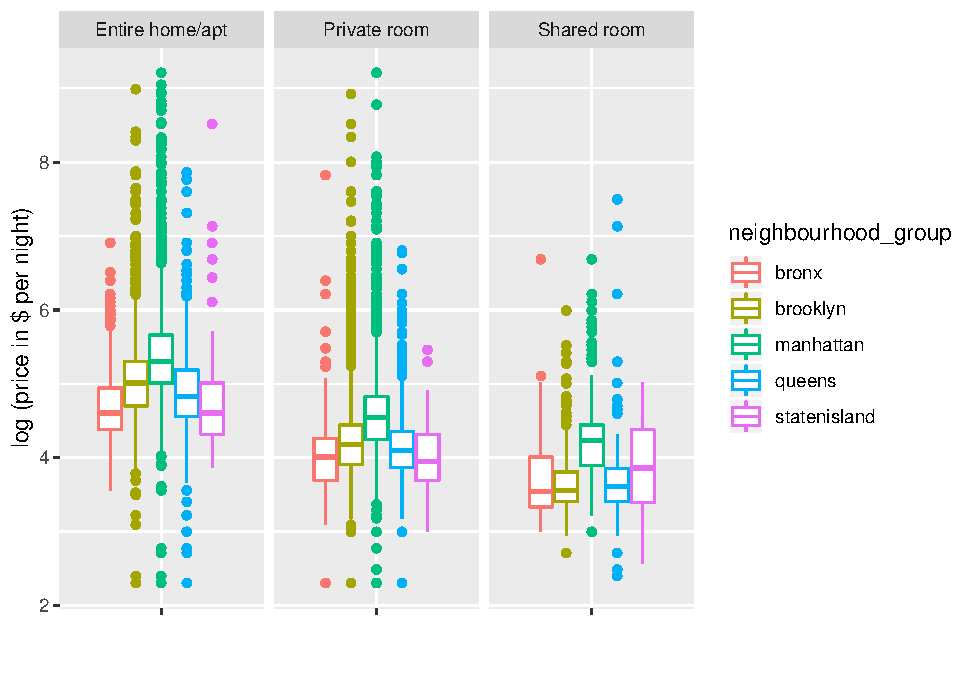
\includegraphics{airbnb_main_files/figure-latex/plot1-1.pdf}

Prices of the room type ``entire home/apt'' have the highest median,
followed by ``private room''" and lastly ``shared room''``, which is not
surprising. 25. and 75. quantile for''entire home/apt" and ``private
room'' are similarly distributed, for shared room there is no clear
pattern.

For all room types, median prices in neighbourhood ``Manhattan'' are the
highest. For for ``entire home/apt'' and ``private room'' the second
highest mediam prices are in Manhattan.

\hypertarget{distribution-of-prices}{%
\subsection{Distribution of prices}\label{distribution-of-prices}}

\begin{Shaded}
\begin{Highlighting}[]
\KeywordTok{ggplot}\NormalTok{(}\DataTypeTok{data =}\NormalTok{ AB_NYC,}
       \DataTypeTok{mapping =} \KeywordTok{aes}\NormalTok{(}\DataTypeTok{x =}\NormalTok{ price_log,}
                     \DataTypeTok{group =}\NormalTok{ room_type,}
                     \DataTypeTok{colour =}\NormalTok{ room_type,}
                     \DataTypeTok{fill =}\NormalTok{ room_type,}
                     \DataTypeTok{alpha =} \FloatTok{0.5}\NormalTok{)) }\OperatorTok{+}
\StringTok{  }\KeywordTok{geom_density}\NormalTok{() }\OperatorTok{+}
\StringTok{  }\KeywordTok{xlab}\NormalTok{(}\StringTok{"log (price in $ per night)"}\NormalTok{)}\OperatorTok{+}
\StringTok{  }\KeywordTok{ylab}\NormalTok{(}\StringTok{"density "}\NormalTok{)}
\end{Highlighting}
\end{Shaded}

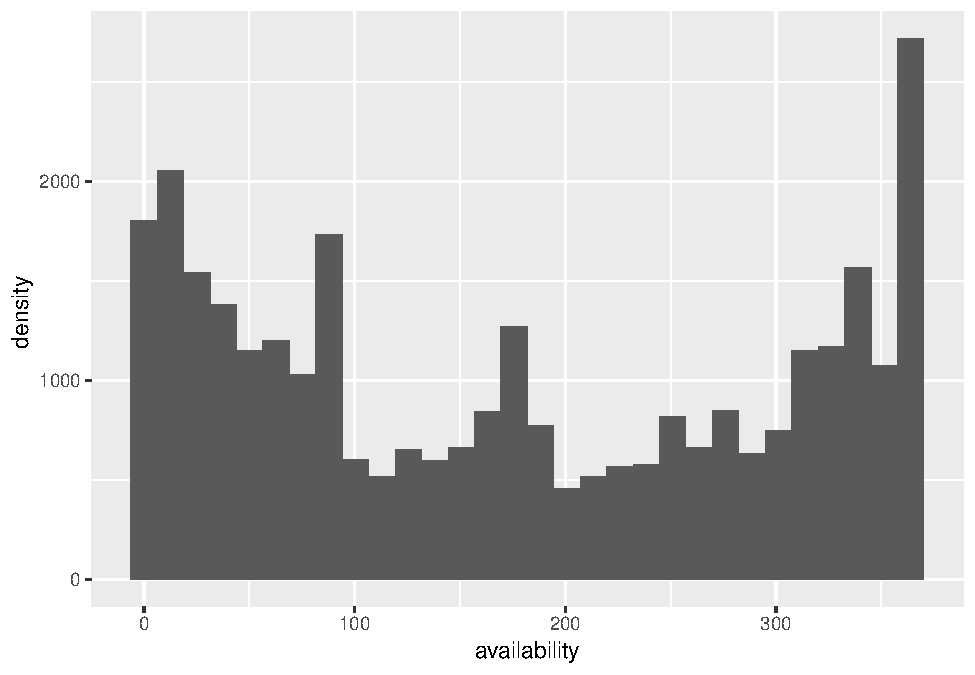
\includegraphics{airbnb_main_files/figure-latex/unnamed-chunk-6-1.pdf}
Prices for all room types are skewed to the right. Even with logarithmic
display of prices, this is still clearly the case.

\hypertarget{availability-of-appartments}{%
\subsection{Availability of
appartments}\label{availability-of-appartments}}

\begin{Shaded}
\begin{Highlighting}[]
\KeywordTok{ggplot}\NormalTok{(}\DataTypeTok{data =}\NormalTok{ AB_NYC_available,}
       \DataTypeTok{mapping =} \KeywordTok{aes}\NormalTok{(}\DataTypeTok{x =}\NormalTok{ availability_}\DecValTok{365}\NormalTok{)) }\OperatorTok{+}
\StringTok{  }\KeywordTok{geom_histogram}\NormalTok{() }\OperatorTok{+}
\StringTok{  }\KeywordTok{xlab}\NormalTok{(}\StringTok{"availability"}\NormalTok{)}\OperatorTok{+}
\StringTok{  }\KeywordTok{ylab}\NormalTok{(}\StringTok{"density "}\NormalTok{)}
\end{Highlighting}
\end{Shaded}

\begin{verbatim}
## `stat_bin()` using `bins = 30`. Pick better value with `binwidth`.
\end{verbatim}

\includegraphics{airbnb_main_files/figure-latex/unnamed-chunk-7-1.pdf}

There are a lot of listings with very low or very high (almost year
round) availablity. Listings with no available days in 2019 were removed
from the dataset. This distribution was not taken into account when
looking at the prices.

\hypertarget{possible-models-to-calculate-the-price-of-an-airbnb}{%
\section{Possible models to calculate the price of an
airbnb}\label{possible-models-to-calculate-the-price-of-an-airbnb}}

\hypertarget{simple-linear-models}{%
\subsection{Simple linear models}\label{simple-linear-models}}

Impact of several variables on the price are analysed. The highest R2 is
reached with ``room type''.

\begin{Shaded}
\begin{Highlighting}[]
\CommentTok{##simple linear models}

\CommentTok{# price ~ neighbourhood group}

\NormalTok{lm.hood <-}\StringTok{ }\KeywordTok{lm}\NormalTok{ (}\DataTypeTok{data=}\NormalTok{AB_NYC_available, price_log}\OperatorTok{~}\NormalTok{neighbourhood_group)}
\KeywordTok{summary}\NormalTok{(lm.hood)}
\end{Highlighting}
\end{Shaded}

\begin{verbatim}
## 
## Call:
## lm(formula = price_log ~ neighbourhood_group, data = AB_NYC_available)
## 
## Residuals:
##     Min      1Q  Median      3Q     Max 
## -2.7663 -0.4698 -0.0473  0.3886  4.3652 
## 
## Coefficients:
##                                 Estimate Std. Error t value Pr(>|t|)    
## (Intercept)                      4.25517    0.02199 193.516  < 2e-16 ***
## neighbourhood_groupbrooklyn      0.36688    0.02279  16.096  < 2e-16 ***
## neighbourhood_groupmanhattan     0.81367    0.02272  35.818  < 2e-16 ***
## neighbourhood_groupqueens        0.12670    0.02421   5.233 1.68e-07 ***
## neighbourhood_groupstatenisland  0.10551    0.04263   2.475   0.0133 *  
## ---
## Signif. codes:  0 '***' 0.001 '**' 0.01 '*' 0.05 '.' 0.1 ' ' 1
## 
## Residual standard error: 0.6644 on 31349 degrees of freedom
## Multiple R-squared:  0.1491, Adjusted R-squared:  0.1489 
## F-statistic:  1373 on 4 and 31349 DF,  p-value: < 2.2e-16
\end{verbatim}

\begin{Shaded}
\begin{Highlighting}[]
\CommentTok{# price ~ room type}

\NormalTok{lm.type <-}\StringTok{ }\KeywordTok{lm}\NormalTok{ (}\DataTypeTok{data=}\NormalTok{AB_NYC_available, price_log}\OperatorTok{~}\NormalTok{room_type)}
\KeywordTok{summary}\NormalTok{(lm.type)}
\end{Highlighting}
\end{Shaded}

\begin{verbatim}
## 
## Call:
## lm(formula = price_log ~ room_type, data = AB_NYC_available)
## 
## Residuals:
##     Min      1Q  Median      3Q     Max 
## -2.8872 -0.3695 -0.0658  0.2816  4.8867 
## 
## Coefficients:
##                        Estimate Std. Error t value Pr(>|t|)    
## (Intercept)            5.189793   0.004377 1185.79   <2e-16 ***
## room_typePrivate room -0.866270   0.006468 -133.92   <2e-16 ***
## room_typeShared room  -1.280409   0.019660  -65.13   <2e-16 ***
## ---
## Signif. codes:  0 '***' 0.001 '**' 0.01 '*' 0.05 '.' 0.1 ' ' 1
## 
## Residual standard error: 0.5627 on 31351 degrees of freedom
## Multiple R-squared:  0.3895, Adjusted R-squared:  0.3895 
## F-statistic: 1e+04 on 2 and 31351 DF,  p-value: < 2.2e-16
\end{verbatim}

\begin{Shaded}
\begin{Highlighting}[]
\CommentTok{# price ~ dist.timessquare}

\NormalTok{lm.dist <-}\StringTok{ }\KeywordTok{lm}\NormalTok{ (}\DataTypeTok{data=}\NormalTok{AB_NYC_available, price_log}\OperatorTok{~}\NormalTok{dist.timessquare)}
\KeywordTok{summary}\NormalTok{(lm.dist)}
\end{Highlighting}
\end{Shaded}

\begin{verbatim}
## 
## Call:
## lm(formula = price_log ~ dist.timessquare, data = AB_NYC_available)
## 
## Residuals:
##     Min      1Q  Median      3Q     Max 
## -2.8052 -0.4752 -0.0408  0.3890  4.4443 
## 
## Coefficients:
##                    Estimate Std. Error t value Pr(>|t|)    
## (Intercept)       5.211e+00  6.900e-03  755.27   <2e-16 ***
## dist.timessquare -5.913e-05  7.753e-07  -76.26   <2e-16 ***
## ---
## Signif. codes:  0 '***' 0.001 '**' 0.01 '*' 0.05 '.' 0.1 ' ' 1
## 
## Residual standard error: 0.6615 on 31352 degrees of freedom
## Multiple R-squared:  0.1565, Adjusted R-squared:  0.1565 
## F-statistic:  5816 on 1 and 31352 DF,  p-value: < 2.2e-16
\end{verbatim}

\hypertarget{multiple-linear-model}{%
\subsection{Multiple linear model}\label{multiple-linear-model}}

A linear model using ``distance to timessquare'' and ``room type'' (as
factor) with interactions to calculate the price is applied.

\begin{Shaded}
\begin{Highlighting}[]
\CommentTok{#distance and room type on price (with interaction)}
\NormalTok{lm.dist.type.interact <-}\StringTok{ }\KeywordTok{lm}\NormalTok{ (}\DataTypeTok{data=}\NormalTok{AB_NYC_available, price_log}\OperatorTok{~}\NormalTok{dist.timessquare}\OperatorTok{*}\NormalTok{room_type)}
\KeywordTok{summary}\NormalTok{(lm.dist.type.interact)}
\end{Highlighting}
\end{Shaded}

\begin{verbatim}
## 
## Call:
## lm(formula = price_log ~ dist.timessquare * room_type, data = AB_NYC_available)
## 
## Residuals:
##     Min      1Q  Median      3Q     Max 
## -3.0389 -0.3348 -0.0639  0.2365  4.7750 
## 
## Coefficients:
##                                          Estimate Std. Error t value
## (Intercept)                             5.480e+00  6.991e-03 783.825
## dist.timessquare                       -4.357e-05  8.550e-07 -50.955
## room_typePrivate room                  -7.825e-01  1.148e-02 -68.163
## room_typeShared room                   -1.214e+00  3.403e-02 -35.682
## dist.timessquare:room_typePrivate room -7.460e-07  1.274e-06  -0.586
## dist.timessquare:room_typeShared room  -2.747e-07  3.568e-06  -0.077
##                                        Pr(>|t|)    
## (Intercept)                              <2e-16 ***
## dist.timessquare                         <2e-16 ***
## room_typePrivate room                    <2e-16 ***
## room_typeShared room                     <2e-16 ***
## dist.timessquare:room_typePrivate room    0.558    
## dist.timessquare:room_typeShared room     0.939    
## ---
## Signif. codes:  0 '***' 0.001 '**' 0.01 '*' 0.05 '.' 0.1 ' ' 1
## 
## Residual standard error: 0.5229 on 31348 degrees of freedom
## Multiple R-squared:  0.4729, Adjusted R-squared:  0.4728 
## F-statistic:  5625 on 5 and 31348 DF,  p-value: < 2.2e-16
\end{verbatim}

\begin{Shaded}
\begin{Highlighting}[]
\KeywordTok{ggplot}\NormalTok{(}\DataTypeTok{data =}\NormalTok{ AB_NYC_available,}
       \DataTypeTok{mapping =} \KeywordTok{aes}\NormalTok{(}\DataTypeTok{y =}\NormalTok{ price,}
                     \DataTypeTok{x =}\NormalTok{ dist.timessquare,}
                     \DataTypeTok{colour =}\NormalTok{ room_type,}
                     \DataTypeTok{group =}\NormalTok{ room_type)) }\OperatorTok{+}
\StringTok{  }\KeywordTok{geom_point}\NormalTok{(}\DataTypeTok{alpha =} \FloatTok{0.03}\NormalTok{) }\OperatorTok{+}
\StringTok{  }\KeywordTok{xlab}\NormalTok{(}\StringTok{"distance to timessquare in m"}\NormalTok{)}\OperatorTok{+}
\StringTok{  }\KeywordTok{ylab}\NormalTok{(}\StringTok{"price in $ per night"}\NormalTok{)}\OperatorTok{+}
\StringTok{  }\KeywordTok{ylim}\NormalTok{(}\DecValTok{0}\NormalTok{,}\DecValTok{300}\NormalTok{)}\OperatorTok{+}
\StringTok{  }\KeywordTok{geom_smooth}\NormalTok{(}\DataTypeTok{method=}\StringTok{"lm"}\NormalTok{)}
\end{Highlighting}
\end{Shaded}

\includegraphics{airbnb_main_files/figure-latex/unnamed-chunk-9-1.pdf}

There is a tendency for all room types that the price is lower if the
place is further from Times Square. The interactions are not
significant.

\hypertarget{multiple-linear-model-by-choosing-smallest-rss}{%
\subsection{Multiple linear model by choosing smallest
RSS}\label{multiple-linear-model-by-choosing-smallest-rss}}

A multiple linear model is created. The best model to calculate the
price we can find includes 5 variables:

\begin{itemize}
\tightlist
\item
  room type (factor with 3 levels, entire appartment being the highest
  and shared room the lowest)
\item
  distance to timessquare (negative effect)
\item
  availability (positive effect)
\item
  neighbourhood group (factor with 5 levels, Manhattan being the highest
  and Bronx the lowest)
\item
  minimum nights (negative effect)
\end{itemize}

\begin{Shaded}
\begin{Highlighting}[]
\CommentTok{#full model}
\NormalTok{lm.full <-}\StringTok{ }\KeywordTok{lm}\NormalTok{ (}\DataTypeTok{data=}\NormalTok{AB_NYC_available, price_log}\OperatorTok{~}\NormalTok{room_type}
               \OperatorTok{+}\NormalTok{neighbourhood_group}
               \OperatorTok{+}\NormalTok{minimum_nights}
               \OperatorTok{+}\NormalTok{number_of_reviews}
               \OperatorTok{+}\NormalTok{calculated_host_listings_count}
               \OperatorTok{+}\NormalTok{availability_}\DecValTok{365}
               \OperatorTok{+}\NormalTok{dist.timessquare)}

\CommentTok{#empty model}
\NormalTok{lm.empty <-}\StringTok{ }\KeywordTok{lm}\NormalTok{ (}\DataTypeTok{data=}\NormalTok{AB_NYC_available, price_log}\OperatorTok{~}\OtherTok{NULL}\NormalTok{)}
\KeywordTok{add1}\NormalTok{(lm.empty,}\DataTypeTok{scope=}\NormalTok{lm.full)}

\CommentTok{#choose value with smallest RSS}
\NormalTok{lm}\FloatTok{.1}\NormalTok{ <-}\StringTok{ }\KeywordTok{update}\NormalTok{(lm.empty,.}\OperatorTok{~}\NormalTok{.}\OperatorTok{+}\NormalTok{room_type) }
\KeywordTok{add1}\NormalTok{(lm}\FloatTok{.1}\NormalTok{,}\DataTypeTok{scope=}\NormalTok{lm.full)}
\NormalTok{lm}\FloatTok{.2}\NormalTok{ <-}\StringTok{ }\KeywordTok{update}\NormalTok{(lm}\FloatTok{.1}\NormalTok{,.}\OperatorTok{~}\NormalTok{.}\OperatorTok{+}\NormalTok{dist.timessquare)}
\KeywordTok{add1}\NormalTok{(lm}\FloatTok{.2}\NormalTok{,}\DataTypeTok{scope=}\NormalTok{lm.full)}
\NormalTok{lm}\FloatTok{.3}\NormalTok{ <-}\StringTok{ }\KeywordTok{update}\NormalTok{(lm}\FloatTok{.2}\NormalTok{,.}\OperatorTok{~}\NormalTok{.}\OperatorTok{+}\NormalTok{availability_}\DecValTok{365}\NormalTok{)}
\KeywordTok{add1}\NormalTok{(lm}\FloatTok{.3}\NormalTok{,}\DataTypeTok{scope=}\NormalTok{lm.full)}
\NormalTok{lm}\FloatTok{.4}\NormalTok{ <-}\StringTok{ }\KeywordTok{update}\NormalTok{(lm}\FloatTok{.3}\NormalTok{,.}\OperatorTok{~}\NormalTok{.}\OperatorTok{+}\NormalTok{neighbourhood_group)}
\KeywordTok{add1}\NormalTok{(lm}\FloatTok{.4}\NormalTok{,}\DataTypeTok{scope=}\NormalTok{lm.full)}
\NormalTok{lm}\FloatTok{.5}\NormalTok{ <-}\StringTok{ }\KeywordTok{update}\NormalTok{(lm}\FloatTok{.4}\NormalTok{,.}\OperatorTok{~}\NormalTok{.}\OperatorTok{+}\NormalTok{minimum_nights)}
\KeywordTok{add1}\NormalTok{(lm}\FloatTok{.5}\NormalTok{,}\DataTypeTok{scope=}\NormalTok{lm.full)}
\end{Highlighting}
\end{Shaded}

\begin{Shaded}
\begin{Highlighting}[]
\KeywordTok{summary}\NormalTok{(lm}\FloatTok{.5}\NormalTok{)}
\end{Highlighting}
\end{Shaded}

\begin{verbatim}
## 
## Call:
## lm(formula = price_log ~ room_type + dist.timessquare + availability_365 + 
##     neighbourhood_group + minimum_nights, data = AB_NYC_available)
## 
## Residuals:
##     Min      1Q  Median      3Q     Max 
## -3.0328 -0.3241 -0.0652  0.2332  4.8822 
## 
## Coefficients:
##                                   Estimate Std. Error  t value Pr(>|t|)
## (Intercept)                      5.082e+00  2.077e-02  244.710  < 2e-16
## room_typePrivate room           -7.823e-01  5.995e-03 -130.499  < 2e-16
## room_typeShared room            -1.235e+00  1.785e-02  -69.173  < 2e-16
## dist.timessquare                -3.073e-05  8.321e-07  -36.926  < 2e-16
## availability_365                 6.388e-04  2.311e-05   27.645  < 2e-16
## neighbourhood_groupbrooklyn      1.415e-01  1.779e-02    7.956 1.83e-15
## neighbourhood_groupmanhattan     3.210e-01  1.908e-02   16.821  < 2e-16
## neighbourhood_groupqueens        4.895e-02  1.863e-02    2.627  0.00861
## neighbourhood_groupstatenisland  1.754e-01  3.306e-02    5.304 1.14e-07
## minimum_nights                  -1.930e-03  1.226e-04  -15.741  < 2e-16
##                                    
## (Intercept)                     ***
## room_typePrivate room           ***
## room_typeShared room            ***
## dist.timessquare                ***
## availability_365                ***
## neighbourhood_groupbrooklyn     ***
## neighbourhood_groupmanhattan    ***
## neighbourhood_groupqueens       ** 
## neighbourhood_groupstatenisland ***
## minimum_nights                  ***
## ---
## Signif. codes:  0 '***' 0.001 '**' 0.01 '*' 0.05 '.' 0.1 ' ' 1
## 
## Residual standard error: 0.5089 on 31344 degrees of freedom
## Multiple R-squared:  0.5009, Adjusted R-squared:  0.5008 
## F-statistic:  3496 on 9 and 31344 DF,  p-value: < 2.2e-16
\end{verbatim}

\hypertarget{interactive-map-with-the-leaflet-package}{%
\section{Interactive map with the leaflet
package}\label{interactive-map-with-the-leaflet-package}}

\begin{Shaded}
\begin{Highlighting}[]
\NormalTok{df_exp<-}\KeywordTok{filter}\NormalTok{(NYC,price }\OperatorTok{==}\StringTok{ }\KeywordTok{max}\NormalTok{(price))}
\NormalTok{df_cheap<-}\KeywordTok{filter}\NormalTok{(NYC,price }\OperatorTok{==}\StringTok{ }\KeywordTok{min}\NormalTok{(price))}
\end{Highlighting}
\end{Shaded}


\end{document}
